\documentclass[conference,letterpaper]{IEEEtran}
\IEEEoverridecommandlockouts
\usepackage{cite}
\usepackage{amsmath,amssymb}
\usepackage{graphicx}
\usepackage{booktabs}
\usepackage{array}
\usepackage{xcolor}
\usepackage{url}
\usepackage[hidelinks]{hyperref}

% Every result below is a macro generated from the evaluation outputs
% (make_numbers.py -> numbers.tex for CHB-MIT, make_numbers_s2.py -> numbers_s2.tex for SeizeIT2).
% AUTO-GENERATED by make_numbers.py — do not edit by hand
% source: ../final2
\newcommand{\Pilot}{0}
\newcommand{\PilotNote}{}
\newcommand{\NSubj}{23}
\newcommand{\NRec}{160}
\newcommand{\NSz}{194}
\newcommand{\NHours}{220}
\newcommand{\NColdStart}{15}
\newcommand{\NRecAll}{165}
\newcommand{\NSzAll}{198}
\newcommand{\NHoursAll}{225}
\newcommand{\PyBSens}{5.7\%}
\newcommand{\PyBDet}{11}
\newcommand{\PyBCI}{2--12\%}
\newcommand{\PyBMacro}{10.0\%}
\newcommand{\PyBMacroCI}{3--18\%}
\newcommand{\PyBFAh}{0.32}
\newcommand{\PyBFAday}{8}
\newcommand{\PyBFACI}{0.20--0.48}
\newcommand{\PyBLat}{26.3}
\newcommand{\PyASens}{21.1\%}
\newcommand{\PyADet}{41}
\newcommand{\PyACI}{14--29\%}
\newcommand{\PyAMacro}{25.4\%}
\newcommand{\PyAMacroCI}{15--36\%}
\newcommand{\PyAFAh}{2.82}
\newcommand{\PyAFAday}{68}
\newcommand{\PyAFACI}{2.00--3.86}
\newcommand{\PyALat}{28.4}
\newcommand{\FwBSens}{75.3\%}
\newcommand{\FwBDet}{146}
\newcommand{\FwBCI}{60--94\%}
\newcommand{\FwBMacro}{87.6\%}
\newcommand{\FwBMacroCI}{79--95\%}
\newcommand{\FwBFAh}{18.29}
\newcommand{\FwBFAday}{439}
\newcommand{\FwBFACI}{15.19--21.21}
\newcommand{\FwBLat}{14.5}
\newcommand{\DevASens}{52.1\%}
\newcommand{\DevADet}{101}
\newcommand{\DevACI}{36--74\%}
\newcommand{\DevAMacro}{68.6\%}
\newcommand{\DevAMacroCI}{54--82\%}
\newcommand{\DevAFAh}{0.97}
\newcommand{\DevAFAday}{23}
\newcommand{\DevAFACI}{0.71--1.31}
\newcommand{\DevALat}{22.0}
\newcommand{\DevBSens}{41.8\%}
\newcommand{\DevBDet}{81}
\newcommand{\DevBCI}{26--65\%}
\newcommand{\DevBMacro}{59.5\%}
\newcommand{\DevBMacroCI}{44--74\%}
\newcommand{\DevBFAh}{0.46}
\newcommand{\DevBFAday}{11}
\newcommand{\DevBFACI}{0.25--0.77}
\newcommand{\DevBLat}{23.0}
\newcommand{\DevCSens}{28.4\%}
\newcommand{\DevCDet}{55}
\newcommand{\DevCCI}{15--49\%}
\newcommand{\DevCMacro}{46.1\%}
\newcommand{\DevCMacroCI}{30--62\%}
\newcommand{\DevCFAh}{0.16}
\newcommand{\DevCFAday}{4}
\newcommand{\DevCFACI}{0.05--0.32}
\newcommand{\DevCLat}{29.0}
\newcommand{\LlASens}{25.3\%}
\newcommand{\LlADet}{49}
\newcommand{\LlACI}{15--42\%}
\newcommand{\LlAMacro}{40.1\%}
\newcommand{\LlAMacroCI}{26--55\%}
\newcommand{\LlAFAh}{1.04}
\newcommand{\LlAFAday}{25}
\newcommand{\LlAFACI}{0.72--1.35}
\newcommand{\LlALat}{32.0}
\newcommand{\LlBSens}{21.6\%}
\newcommand{\LlBDet}{42}
\newcommand{\LlBCI}{11--38\%}
\newcommand{\LlBMacro}{35.8\%}
\newcommand{\LlBMacroCI}{21--50\%}
\newcommand{\LlBFAh}{0.35}
\newcommand{\LlBFAday}{8}
\newcommand{\LlBFACI}{0.23--0.51}
\newcommand{\LlBLat}{24.5}
\newcommand{\FuASens}{40.2\%}
\newcommand{\FuADet}{78}
\newcommand{\FuACI}{24--64\%}
\newcommand{\FuAMacro}{56.0\%}
\newcommand{\FuAMacroCI}{41--70\%}
\newcommand{\FuAFAh}{0.96}
\newcommand{\FuAFAday}{23}
\newcommand{\FuAFACI}{0.67--1.27}
\newcommand{\FuALat}{21.5}
\newcommand{\TwoDevASens}{52.1\%}
\newcommand{\TwoDevADet}{101}
\newcommand{\TwoDevACI}{36--74\%}
\newcommand{\TwoDevAMacro}{68.6\%}
\newcommand{\TwoDevAMacroCI}{54--82\%}
\newcommand{\TwoDevAFAh}{0.95}
\newcommand{\TwoDevAFAday}{23}
\newcommand{\TwoDevAFACI}{0.69--1.31}
\newcommand{\TwoDevALat}{23.0}
\newcommand{\TwoDevBSens}{38.1\%}
\newcommand{\TwoDevBDet}{74}
\newcommand{\TwoDevBCI}{24--61\%}
\newcommand{\TwoDevBMacro}{57.3\%}
\newcommand{\TwoDevBMacroCI}{41--73\%}
\newcommand{\TwoDevBFAh}{0.37}
\newcommand{\TwoDevBFAday}{9}
\newcommand{\TwoDevBFACI}{0.23--0.55}
\newcommand{\TwoDevBLat}{27.0}
\newcommand{\NeASens}{52.1\%}
\newcommand{\NeADet}{101}
\newcommand{\NeACI}{36--74\%}
\newcommand{\NeAMacro}{68.6\%}
\newcommand{\NeAMacroCI}{54--82\%}
\newcommand{\NeAFAh}{0.97}
\newcommand{\NeAFAday}{23}
\newcommand{\NeAFACI}{0.71--1.31}
\newcommand{\NeALat}{22.0}
\newcommand{\NeBSens}{41.8\%}
\newcommand{\NeBDet}{81}
\newcommand{\NeBCI}{26--65\%}
\newcommand{\NeBMacro}{59.5\%}
\newcommand{\NeBMacroCI}{44--74\%}
\newcommand{\NeBFAh}{0.46}
\newcommand{\NeBFAday}{11}
\newcommand{\NeBFACI}{0.25--0.77}
\newcommand{\NeBLat}{23.0}
\newcommand{\DevASensWarm}{54.2\%}
\newcommand{\DevASzWarm}{179}
\newcommand{\DevBSensWarm}{43.6\%}
\newcommand{\DevBSzWarm}{179}
\newcommand{\DevAR}{1.25}
\newcommand{\DevAD}{20}
\newcommand{\DevAModeCount}{22}
\newcommand{\DevAFolds}{23}
\newcommand{\DevBR}{1.5}
\newcommand{\DevBD}{20}
\newcommand{\DevBModeCount}{20}
\newcommand{\DevBFolds}{23}
\newcommand{\NestedDev}{69}
\newcommand{\NestedAll}{69}
\newcommand{\PyBNull}{1.6\%}
\newcommand{\PyBNullNF}{3.1\%}
\newcommand{\PyBNullP}{$p{=}1{\times}10^{-3}$}
\newcommand{\PyANull}{12.8\%}
\newcommand{\PyANullNF}{16.5\%}
\newcommand{\PyANullP}{$p{=}0.002$}
\newcommand{\FwBNull}{56.6\%}
\newcommand{\FwBNullNF}{61.3\%}
\newcommand{\FwBNullP}{$p{=}1{\times}10^{-3}$}
\newcommand{\DevANull}{6.5\%}
\newcommand{\DevANullNF}{9.3\%}
\newcommand{\DevANullP}{$p{=}1{\times}10^{-3}$}
\newcommand{\DevBNull}{3.9\%}
\newcommand{\DevBNullNF}{6.2\%}
\newcommand{\DevBNullP}{$p{=}1{\times}10^{-3}$}
\newcommand{\LlANull}{4.8\%}
\newcommand{\LlANullNF}{7.2\%}
\newcommand{\LlANullP}{$p{=}1{\times}10^{-3}$}
\newcommand{\NPerm}{1000}
\newcommand{\ShipNullMaxP}{0.002}
\newcommand{\TestDevPyP}{$p{=}6{\times}10^{-5}$}
\newcommand{\TestDevPyBetter}{21}
\newcommand{\TestDevPyWorse}{0}
\newcommand{\TestDevPyTies}{2}
\newcommand{\TestDevPyN}{23}
\newcommand{\TestDevPyAnyP}{$p{=}7{\times}10^{-5}$}
\newcommand{\TestDevPyAnyBetter}{20}
\newcommand{\TestDevPyAnyWorse}{1}
\newcommand{\TestDevPyAnyTies}{2}
\newcommand{\TestDevPyAnyN}{23}
\newcommand{\TestDevLlP}{$p{=}7{\times}10^{-4}$}
\newcommand{\TestDevLlBetter}{15}
\newcommand{\TestDevLlWorse}{0}
\newcommand{\TestDevLlTies}{8}
\newcommand{\TestDevLlN}{23}
\newcommand{\FoldDevPy}{7}
\newcommand{\AucLL}{0.70}
\newcommand{\AucLLCase}{0.79}
\newcommand{\AucDAR}{0.51}
\newcommand{\AucDARCase}{0.58}
\newcommand{\AucHFE}{0.40}
\newcommand{\AucHFECase}{0.41}
\newcommand{\AucFW}{0.70}
\newcommand{\AucFWCase}{0.83}
\newcommand{\ArtIctal}{0.01\%}
\newcommand{\ArtInter}{0.01\%}
\newcommand{\PyBSensLowGain}{0.0\%}
\newcommand{\PyBSensHighGain}{13.4\%}
\newcommand{\PyBFAhLowGain}{0.24}
\newcommand{\PyBFAhHighGain}{1.59}
\newcommand{\FwBFAhLowGain}{7.36}
\newcommand{\FwBFAhHighGain}{24.37}
\newcommand{\MainTableBody}{%
Analyzer, BLACKOUT (shipped) & 11/194 & 5.7\% [2--12] & 10.0\% & 0.32 & 26.3 & 1.6\% \\
Analyzer, any alarm (shipped) & 41/194 & 21.1\% [14--29] & 25.4\% & 2.82 & 28.4 & 12.8\% \\
Firmware, BLACKOUT (shipped) & 146/194 & 75.3\% [60--94] & 87.6\% & 18.29 & 14.5 & 56.6\% \\
\midrule
LL-BR, $\le$1 FA/h & 49/194 & 25.3\% [15--42] & 40.1\% & 1.04 & 32.0 & 4.8\% \\
FUSE-BR, $\le$1 FA/h & 78/194 & 40.2\% [24--64] & 56.0\% & 0.96 & 21.5 & -- \\
\textbf{DEV-BR, $\le$1 FA/h} & 101/194 & 52.1\% [36--74] & 68.6\% & 0.97 & 22.0 & 6.5\% \\
\textbf{DEV-BR, $\le$0.5 FA/h} & 81/194 & 41.8\% [26--65] & 59.5\% & 0.46 & 23.0 & 3.9\% \\
\textbf{DEV-BR, $\le$0.2 FA/h} & 55/194 & 28.4\% [15--49] & 46.1\% & 0.16 & 29.0 & -- \\
}
\newcommand{\AltBestOneSens}{51.0\%}
\newcommand{\AltBestHalfSens}{44.3\%}
\newcommand{\GbmOneSens}{47.9\%}
\newcommand{\GbmHalfSens}{44.3\%}
\newcommand{\GbmHalfBetter}{4}
\newcommand{\GbmHalfWorse}{2}
\newcommand{\GbmHalfP}{$p{=}0.25$}
\newcommand{\AblationTableBody}{%
\textbf{reference} (300 s, lag 30 s, median) & 52.1\% / 0.97 & 41.8\% / 0.46 \\
no lag (0 s) & 50.5\% / 0.79 & 34.5\% / 0.42 \\
lag 10 s & 51.0\% / 0.87 & 40.7\% / 0.45 \\
lag 60 s & 47.9\% / 0.93 & 38.7\% / 0.46 \\
window 60 s & 50.5\% / 0.94 & 43.3\% / 0.45 \\
window 120 s & 53.1\% / 0.88 & 38.1\% / 0.43 \\
window 600 s & 41.2\% / 0.94 & 34.0\% / 0.47 \\
mean instead of median & 50.0\% / 0.78 & 41.2\% / 0.35 \\
no normalization (absolute) & 32.5\% / 0.83 & 30.4\% / 0.42 \\
\midrule
k-of-n persistence & 43.3\% / 0.95 & 36.6\% / 0.38 \\
dual time-scale rule & 51.0\% / 1.01 & 42.8\% / 0.49 \\
baseline carried across files & 48.5\% / 0.97 & 41.8\% / 0.46 \\
log.\ regression, firmware features & 43.3\% / 1.03 & 35.1\% / 0.44 \\
log.\ regression, all features & 43.8\% / 0.90 & 38.7\% / 0.47 \\
boosted trees, all features & 47.9\% / 1.01 & 44.3\% / 0.50 \\
}
\newcommand{\AblAbsSens}{32.5\%}
\newcommand{\AblLagZeroSensB}{34.5\%}
\newcommand{\AblMeanSens}{50.0\%}
\newcommand{\AblWinLongSens}{41.2\%}
\newcommand{\DevSensOne}{44.4\%}
\newcommand{\SecLlPOne}{$p{=}0.061$}
\newcommand{\SecNestedDevOne}{67}
\newcommand{\DevSensTwo}{39.9\%}
\newcommand{\SecLlPTwo}{$p{=}0.055$}
\newcommand{\SecNestedDevTwo}{63}
\newcommand{\SecondaryTableBody}{%
FP1-F7 & 28.3\% / 4.01 & 77.3\% / 24.42 & 33.8\% / 0.95 & 44.4\% / 0.78 \\
FP2-F8 & 29.3\% / 3.83 & 82.8\% / 24.79 & 27.3\% / 0.89 & 39.9\% / 0.86 \\
}
\newcommand{\HwAvailable}{1}
\newcommand{\HwTableBody}{%
$\times$500 & 0.00\% & 52.1\% / 0.98 & 47.9\% / 0.94 & 51.5\% / 7.36 \\
$\times$1000 (ref.) & 0.00\% & 52.1\% / 0.95 & 52.1\% / 0.97 & 75.3\% / 18.29 \\
$\times$2000 & 0.01\% & 52.1\% / 0.97 & 50.0\% / 0.96 & 86.1\% / 24.37 \\
$\times$1000, LM358 clip & 0.52\% & 51.5\% / 0.97 & 48.5\% / 0.96 & 73.2\% / 18.01 \\
$\times$2000, LM358 clip & 2.69\% & 50.0\% / 0.93 & 50.0\% / 0.93 & 82.0\% / 23.09 \\
$\times$1000, 3.1-V ADC & 0.00\% & 52.1\% / 0.96 & 50.5\% / 0.98 & 78.9\% / 19.22 \\
$\times$1000, 167-Hz loop & 0.00\% & 51.5\% / 0.95 & 51.5\% / 0.96 & 45.9\% / 14.74 \\
}
\newcommand{\HwFixR}{1.25}
\newcommand{\HwFixD}{20}
\newcommand{\HwDevSensMin}{50.0\%}
\newcommand{\HwDevSensMax}{52.1\%}
\newcommand{\HwDevFAMin}{0.93}
\newcommand{\HwDevFAMax}{0.98}
\newcommand{\HwFwSensMin}{45.9\%}
\newcommand{\HwFwSensMax}{86.1\%}
\newcommand{\HwFwFAMin}{7.36}
\newcommand{\HwFwFAMax}{24.37}
\newcommand{\HwGainSens}{52.1\%}
\newcommand{\HwClipSat}{2.7\%}
\newcommand{\HwClipSens}{50.0\%}

% AUTO-GENERATED by make_numbers_s2.py — do not edit by hand
\newcommand{\SNSubj}{125}
\newcommand{\SNRuns}{2850}
\newcommand{\SNSz}{883}
\newcommand{\SHours}{11{,}626}
\newcommand{\SMovMissing}{386}
\newcommand{\SNMotor}{371}
\newcommand{\SNNonMotor}{324}
\newcommand{\SNFBTC}{55}
\newcommand{\SNOther}{133}
\newcommand{\SFwTarget}{7.01}
\newcommand{\SNSleep}{367}
\newcommand{\SFwSens}{57.0\%}
\newcommand{\SFwDet}{503}
\newcommand{\SFwFAh}{7.01}
\newcommand{\SFwFAday}{168.2}
\newcommand{\SFwMacro}{59.5\%}
\newcommand{\SFwCI}{47--65\%}
\newcommand{\SFwLat}{18.1}
\newcommand{\SFwMot}{55.3\%}
\newcommand{\SFwNonMot}{54.6\%}
\newcommand{\SFwFBTC}{87.3\%}
\newcommand{\SFwSleep}{64.0\%}
\newcommand{\SFwAwake}{58.0\%}
\newcommand{\SFwNull}{29.9\%}
\newcommand{\SFwNullP}{$p{=}0.005$}
\newcommand{\SEegASens}{33.1\%}
\newcommand{\SEegADet}{292}
\newcommand{\SEegAFAh}{0.93}
\newcommand{\SEegAFAday}{22.3}
\newcommand{\SEegAMacro}{47.6\%}
\newcommand{\SEegACI}{23--44\%}
\newcommand{\SEegALat}{40.0}
\newcommand{\SEegAMot}{41.8\%}
\newcommand{\SEegANonMot}{16.0\%}
\newcommand{\SEegAFBTC}{92.7\%}
\newcommand{\SEegASleep}{32.2\%}
\newcommand{\SEegAAwake}{36.2\%}
\newcommand{\SEegANull}{4.7\%}
\newcommand{\SEegANullP}{$p{=}0.005$}
\newcommand{\SEegBSens}{24.0\%}
\newcommand{\SEegBDet}{212}
\newcommand{\SEegBFAh}{0.47}
\newcommand{\SEegBFAday}{11.3}
\newcommand{\SEegBMacro}{36.4\%}
\newcommand{\SEegBCI}{15--35\%}
\newcommand{\SEegBLat}{44.0}
\newcommand{\SEegBMot}{28.6\%}
\newcommand{\SEegBNonMot}{9.3\%}
\newcommand{\SEegBFBTC}{92.7\%}
\newcommand{\SEegBSleep}{23.7\%}
\newcommand{\SEegBAwake}{25.4\%}
\newcommand{\SEegBNull}{2.8\%}
\newcommand{\SEegBNullP}{$p{=}0.005$}
\newcommand{\SEegCSens}{14.4\%}
\newcommand{\SEegCDet}{127}
\newcommand{\SEegCFAh}{0.22}
\newcommand{\SEegCFAday}{5.3}
\newcommand{\SEegCMacro}{24.9\%}
\newcommand{\SEegCCI}{8--24\%}
\newcommand{\SEegCLat}{47.0}
\newcommand{\SEegCMot}{13.7\%}
\newcommand{\SEegCNonMot}{2.8\%}
\newcommand{\SEegCFBTC}{89.1\%}
\newcommand{\SEegCSleep}{16.1\%}
\newcommand{\SEegCAwake}{13.1\%}
\newcommand{\SMovASens}{28.3\%}
\newcommand{\SMovADet}{250}
\newcommand{\SMovAFAh}{1.00}
\newcommand{\SMovAFAday}{24.0}
\newcommand{\SMovAMacro}{42.8\%}
\newcommand{\SMovACI}{22--36\%}
\newcommand{\SMovALat}{33.0}
\newcommand{\SMovAMot}{39.1\%}
\newcommand{\SMovANonMot}{10.8\%}
\newcommand{\SMovAFBTC}{90.9\%}
\newcommand{\SMovASleep}{28.3\%}
\newcommand{\SMovAAwake}{31.0\%}
\newcommand{\SMovANull}{4.3\%}
\newcommand{\SMovANullP}{$p{=}0.005$}
\newcommand{\SMovBSens}{16.1\%}
\newcommand{\SMovBDet}{142}
\newcommand{\SMovBFAh}{0.49}
\newcommand{\SMovBFAday}{11.8}
\newcommand{\SMovBMacro}{31.0\%}
\newcommand{\SMovBCI}{11--22\%}
\newcommand{\SMovBLat}{44.5}
\newcommand{\SMovBMot}{18.9\%}
\newcommand{\SMovBNonMot}{4.3\%}
\newcommand{\SMovBFBTC}{89.1\%}
\newcommand{\SMovBSleep}{15.0\%}
\newcommand{\SMovBAwake}{18.8\%}
\newcommand{\SMovBNull}{2.0\%}
\newcommand{\SMovBNullP}{$p{=}0.005$}
\newcommand{\SMovCSens}{9.9\%}
\newcommand{\SMovCDet}{87}
\newcommand{\SMovCFAh}{0.23}
\newcommand{\SMovCFAday}{5.5}
\newcommand{\SMovCMacro}{21.3\%}
\newcommand{\SMovCCI}{6--14\%}
\newcommand{\SMovCLat}{47.0}
\newcommand{\SMovCMot}{9.4\%}
\newcommand{\SMovCNonMot}{1.5\%}
\newcommand{\SMovCFBTC}{81.8\%}
\newcommand{\SMovCSleep}{9.8\%}
\newcommand{\SMovCAwake}{11.3\%}
\newcommand{\SFusASens}{31.1\%}
\newcommand{\SFusADet}{275}
\newcommand{\SFusAFAh}{0.97}
\newcommand{\SFusAFAday}{23.2}
\newcommand{\SFusAMacro}{43.5\%}
\newcommand{\SFusACI}{22--42\%}
\newcommand{\SFusALat}{33.0}
\newcommand{\SFusAMot}{36.7\%}
\newcommand{\SFusANonMot}{15.7\%}
\newcommand{\SFusAFBTC}{96.4\%}
\newcommand{\SFusASleep}{32.2\%}
\newcommand{\SFusAAwake}{32.2\%}
\newcommand{\SFusANull}{4.7\%}
\newcommand{\SFusANullP}{$p{=}0.005$}
\newcommand{\SFusBSens}{24.0\%}
\newcommand{\SFusBDet}{212}
\newcommand{\SFusBFAh}{0.49}
\newcommand{\SFusBFAday}{11.7}
\newcommand{\SFusBMacro}{36.4\%}
\newcommand{\SFusBCI}{15--35\%}
\newcommand{\SFusBLat}{44.0}
\newcommand{\SFusBMot}{28.6\%}
\newcommand{\SFusBNonMot}{9.3\%}
\newcommand{\SFusBFBTC}{92.7\%}
\newcommand{\SFusBSleep}{23.7\%}
\newcommand{\SFusBAwake}{25.4\%}
\newcommand{\SFusBNull}{2.8\%}
\newcommand{\SFusBNullP}{$p{=}0.005$}
\newcommand{\SFusCSens}{14.4\%}
\newcommand{\SFusCDet}{127}
\newcommand{\SFusCFAh}{0.23}
\newcommand{\SFusCFAday}{5.5}
\newcommand{\SFusCMacro}{25.3\%}
\newcommand{\SFusCCI}{8--24\%}
\newcommand{\SFusCLat}{47.0}
\newcommand{\SFusCMot}{13.7\%}
\newcommand{\SFusCNonMot}{2.8\%}
\newcommand{\SFusCFBTC}{90.9\%}
\newcommand{\SFusCSleep}{16.3\%}
\newcommand{\SFusCAwake}{12.9\%}
\newcommand{\SCoASens}{33.6\%}
\newcommand{\SCoADet}{297}
\newcommand{\SCoAFAh}{0.79}
\newcommand{\SCoAFAday}{18.9}
\newcommand{\SCoAMacro}{43.4\%}
\newcommand{\SCoACI}{24--45\%}
\newcommand{\SCoALat}{35.0}
\newcommand{\SCoAMot}{41.8\%}
\newcommand{\SCoANonMot}{14.5\%}
\newcommand{\SCoAFBTC}{92.7\%}
\newcommand{\SCoASleep}{35.7\%}
\newcommand{\SCoAAwake}{35.2\%}
\newcommand{\SCoANull}{3.9\%}
\newcommand{\SCoANullP}{$p{=}0.005$}
\newcommand{\SCoBSens}{25.6\%}
\newcommand{\SCoBDet}{226}
\newcommand{\SCoBFAh}{0.46}
\newcommand{\SCoBFAday}{11.1}
\newcommand{\SCoBMacro}{36.3\%}
\newcommand{\SCoBCI}{17--36\%}
\newcommand{\SCoBLat}{36.0}
\newcommand{\SCoBMot}{29.4\%}
\newcommand{\SCoBNonMot}{10.8\%}
\newcommand{\SCoBFBTC}{92.7\%}
\newcommand{\SCoBSleep}{28.1\%}
\newcommand{\SCoBAwake}{26.1\%}
\newcommand{\SCoBNull}{2.4\%}
\newcommand{\SCoBNullP}{$p{=}0.005$}
\newcommand{\SGyrASens}{21.0\%}
\newcommand{\SGyrADet}{185}
\newcommand{\SGyrAFAh}{0.91}
\newcommand{\SGyrAFAday}{21.8}
\newcommand{\SGyrAMacro}{28.2\%}
\newcommand{\SGyrACI}{15--29\%}
\newcommand{\SGyrALat}{38.0}
\newcommand{\SGyrAMot}{24.8\%}
\newcommand{\SGyrANonMot}{10.5\%}
\newcommand{\SGyrAFBTC}{74.5\%}
\newcommand{\SGyrASleep}{18.8\%}
\newcommand{\SGyrAAwake}{24.9\%}
\newcommand{\SGyrANull}{3.8\%}
\newcommand{\SGyrANullP}{$p{=}0.005$}
\newcommand{\SGyrBSens}{15.5\%}
\newcommand{\SGyrBDet}{137}
\newcommand{\SGyrBFAh}{0.49}
\newcommand{\SGyrBFAday}{11.8}
\newcommand{\SGyrBMacro}{22.4\%}
\newcommand{\SGyrBCI}{11--21\%}
\newcommand{\SGyrBLat}{40.0}
\newcommand{\SGyrBMot}{17.8\%}
\newcommand{\SGyrBNonMot}{6.8\%}
\newcommand{\SGyrBFBTC}{69.1\%}
\newcommand{\SGyrBSleep}{16.3\%}
\newcommand{\SGyrBAwake}{16.0\%}
\newcommand{\SGyrBNull}{2.2\%}
\newcommand{\SGyrBNullP}{$p{=}0.005$}
\newcommand{\SEegFwSens}{63.2\%}
\newcommand{\SEegFwDet}{558}
\newcommand{\SEegFwFAh}{5.73}
\newcommand{\SEegFwFAday}{137.4}
\newcommand{\SEegFwMacro}{70.3\%}
\newcommand{\SEegFwCI}{54--72\%}
\newcommand{\SEegFwLat}{18.0}
\newcommand{\SEegFwMot}{74.7\%}
\newcommand{\SEegFwNonMot}{47.8\%}
\newcommand{\SEegFwFBTC}{94.5\%}
\newcommand{\SEegFwSleep}{70.8\%}
\newcommand{\SEegFwAwake}{62.9\%}
\newcommand{\SFusFwSens}{68.7\%}
\newcommand{\SFusFwDet}{607}
\newcommand{\SFusFwFAh}{6.28}
\newcommand{\SFusFwFAday}{150.7}
\newcommand{\SFusFwMacro}{74.6\%}
\newcommand{\SFusFwCI}{57--79\%}
\newcommand{\SFusFwLat}{14.0}
\newcommand{\SFusFwMot}{80.1\%}
\newcommand{\SFusFwNonMot}{53.4\%}
\newcommand{\SFusFwFBTC}{98.2\%}
\newcommand{\SFusFwSleep}{83.1\%}
\newcommand{\SFusFwAwake}{63.6\%}
\newcommand{\STFUSEDBVEEGBBetter}{0}
\newcommand{\STFUSEDBVEEGBWorse}{0}
\newcommand{\STFUSEDBVEEGBP}{$p{=}1.000$}
\newcommand{\STFUSEDBVMOVBBetter}{36}
\newcommand{\STFUSEDBVMOVBWorse}{15}
\newcommand{\STFUSEDBVMOVBP}{$p{=}0.025$}
\newcommand{\STMOVBVEEGBBetter}{15}
\newcommand{\STMOVBVEEGBWorse}{36}
\newcommand{\STMOVBVEEGBP}{$p{=}0.025$}
\newcommand{\STEEGBVFWBetter}{11}
\newcommand{\STEEGBVFWWorse}{64}
\newcommand{\STEEGBVFWP}{$p{=}8{\times}10^{-8}$}
\newcommand{\STCOACTBVEEGBBetter}{19}
\newcommand{\STCOACTBVEEGBWorse}{15}
\newcommand{\STCOACTBVEEGBP}{$p{=}0.939$}
\newcommand{\STFUSEDBVFWBetter}{11}
\newcommand{\STFUSEDBVFWWorse}{64}
\newcommand{\STFUSEDBVFWP}{$p{=}8{\times}10^{-8}$}
\newcommand{\STFUSEDAVEEGABetter}{13}
\newcommand{\STFUSEDAVEEGAWorse}{26}
\newcommand{\STFUSEDAVEEGAP}{$p{=}0.059$}
\newcommand{\STFUSEDAVMOVABetter}{35}
\newcommand{\STFUSEDAVMOVAWorse}{30}
\newcommand{\STFUSEDAVMOVAP}{$p{=}0.621$}
\newcommand{\STMOVAVEEGABetter}{23}
\newcommand{\STMOVAVEEGAWorse}{40}
\newcommand{\STMOVAVEEGAP}{$p{=}0.073$}
\newcommand{\STEEGAVFWBetter}{23}
\newcommand{\STEEGAVFWWorse}{53}
\newcommand{\STEEGAVFWP}{$p{=}0.002$}
\newcommand{\STCOACTAVEEGABetter}{22}
\newcommand{\STCOACTAVEEGAWorse}{28}
\newcommand{\STCOACTAVEEGAP}{$p{=}0.122$}
\newcommand{\STFUSEDAVFWBetter}{17}
\newcommand{\STFUSEDAVFWWorse}{55}
\newcommand{\STFUSEDAVFWP}{$p{=}6{\times}10^{-5}$}
\newcommand{\STEEGFwVFWBetter}{46}
\newcommand{\STEEGFwVFWWorse}{20}
\newcommand{\STEEGFwVFWP}{$p{=}0.002$}
\newcommand{\STFUSEDFwVFWBetter}{53}
\newcommand{\STFUSEDFwVFWWorse}{21}
\newcommand{\STFUSEDFwVFWP}{$p{=}4{\times}10^{-5}$}
\newcommand{\SVerRuns}{2850}
\newcommand{\SVerSame}{2850}
\newcommand{\SVerAlarms}{11{,}743}
\newcommand{\SVerNote}{(2850 of 2850 SeizeIT2 recordings identical, 11{,}743 alarms)}
\newcommand{\SCvADet}{42}
\newcommand{\SCvAN}{55}
\newcommand{\SCvASens}{76.4\%}
\newcommand{\SCvACI}{63--88\%}
\newcommand{\SCvASubj}{37}
\newcommand{\SCvAFAday}{0.48}
\newcommand{\SCvALat}{72}
\newcommand{\SCvALatIQR}{50--97}
\newcommand{\SCvASleepDet}{20}
\newcommand{\SCvASleepN}{25}
\newcommand{\SCvAZeroFA}{69}
\newcommand{\SCvEegDet}{17}
\newcommand{\SCvEegN}{55}
\newcommand{\SCvEegSens}{30.9\%}
\newcommand{\SCvEegCI}{15--47\%}
\newcommand{\SCvEegSubj}{37}
\newcommand{\SCvEegFAday}{0.47}
\newcommand{\SCvEegLat}{86}
\newcommand{\SCvEegLatIQR}{62--99}
\newcommand{\SCvEegSleepDet}{12}
\newcommand{\SCvEegSleepN}{25}
\newcommand{\SCvEegZeroFA}{63}
\newcommand{\SCvMovDet}{13}
\newcommand{\SCvMovN}{55}
\newcommand{\SCvMovSens}{23.6\%}
\newcommand{\SCvMovCI}{13--35\%}
\newcommand{\SCvMovSubj}{37}
\newcommand{\SCvMovFAday}{0.45}
\newcommand{\SCvMovLat}{101}
\newcommand{\SCvMovLatIQR}{91--120}
\newcommand{\SCvMovSleepDet}{4}
\newcommand{\SCvMovSleepN}{25}
\newcommand{\SCvMovZeroFA}{84}
\newcommand{\SCvBDet}{46}
\newcommand{\SCvBN}{55}
\newcommand{\SCvBSens}{83.6\%}
\newcommand{\SCvBCI}{71--94\%}
\newcommand{\SCvBSubj}{37}
\newcommand{\SCvBFAday}{0.91}
\newcommand{\SCvBLat}{64}
\newcommand{\SCvBLatIQR}{44--79}
\newcommand{\SCvBSleepDet}{21}
\newcommand{\SCvBSleepN}{25}
\newcommand{\SCvBZeroFA}{46}
\newcommand{\SMcEegOnly}{26}
\newcommand{\SMcEegOther}{1}
\newcommand{\SMcEegP}{$p{=}4{\times}10^{-7}$}
\newcommand{\SMcMovOnly}{30}
\newcommand{\SMcMovOther}{1}
\newcommand{\SMcMovP}{$p{=}3{\times}10^{-8}$}
\newcommand{\SCvAParamsN}{122}
\newcommand{\SFusAParamsN}{106}
\newcommand{\SMainTableBody}{%
Shipped firmware (BLACKOUT) & 503/883 & 57.0\% [47--65] & 7.01 & 87.3\% & 55.3\% & 54.6\% & 64.0\% & 29.9\% \\
\multicolumn{9}{l}{\textit{Same false-alarm rate as the shipped firmware}} \\
EEG: DEV-BR & 558/883 & 63.2\% [54--72] & 5.73 & 94.5\% & 74.7\% & 47.8\% & 70.8\% & -- \\
EEG or motion & 607/883 & 68.7\% [57--79] & 6.28 & 98.2\% & 80.1\% & 53.4\% & 83.1\% & -- \\
\multicolumn{9}{l}{\textit{General mode, $\le$1 FA/h target}} \\
EEG: DEV-BR & 292/883 & 33.1\% [23--44] & 0.93 & 92.7\% & 41.8\% & 16.0\% & 32.2\% & 4.7\% \\
Motion: MOV-BR & 250/883 & 28.3\% [22--36] & 1.00 & 90.9\% & 39.1\% & 10.8\% & 28.3\% & 4.3\% \\
EEG or motion & 275/883 & 31.1\% [22--42] & 0.97 & 96.4\% & 36.7\% & 15.7\% & 32.2\% & 4.7\% \\
\multicolumn{9}{l}{\textit{Convulsive mode, chosen for FBTC at $\le$0.02 FA/h ($\approx$0.5/day)}} \\
EEG only & 21/883 & 2.4\% [1--4] & 0.020 & 30.9\% & 0.5\% & 0.0\% & 3.8\% & 0.2\% \\
Motion only & 14/883 & 1.6\% [1--3] & 0.019 & 23.6\% & 0.0\% & 0.3\% & 1.4\% & 0.1\% \\
\textbf{EEG AND motion} & 75/883 & 8.5\% [4--15] & 0.020 & 76.4\% & 5.4\% & 1.2\% & 11.2\% & 0.4\% \\
}


\begin{document}

\title{A Low-Cost EEG and Head-Motion Seizure Alarm: Code-Faithful Evaluation and an Embedded Multimodal Detector}

\author{
\IEEEauthorblockN{Sharan Tangalapally}
\IEEEauthorblockA{\textit{VNR Vignana Jyothi Institute of Engineering and Technology}\\
Hyderabad, India\\
shwethasharan.office@gmail.com}
\and
\IEEEauthorblockN{Vedanti Renghe}
\IEEEauthorblockA{\textit{Terna Medical College}\\
Navi Mumbai, India\\
vedantimr@gmail.com}
}

\maketitle

\begin{abstract}
Home seizure alarms built from low-cost amplifiers and microcontrollers are rarely tested against annotated seizures. We describe an open-source wearable combining single-channel EEG (EXG BioAmp Pill) and an MPU9250 head-motion sensor on an ESP32, and evaluate its firmware by \emph{code-faithful replay} of public recordings through the device's signal chain. On CHB-MIT (\NSubj{} subjects, exact FP1--FP2 montage) the shipped detectors were near chance, while a delayed-median ratio rule on the firmware's own EEG deviation (DEV-BR) detected \DevASens{} of seizures at \DevAFAh{} false alarms per hour (FA/h) in held-out subjects, unaffected by gain, clipping and sampling errors. On SeizeIT2 (\SNSubj{} patients, \SHours{}~h, \SNSz{} seizures), requiring EEG \emph{and} head motion to rise together detected \SCvASens{} (95\% CI \SCvACI{}) of focal-to-bilateral tonic--clonic seizures at \SCvAFAday{} false alarms per day, versus \SCvEegSens{} for EEG and \SCvMovSens{} for motion alone. The detectors need under 7~KB of RAM and the v5 firmware reproduces the evaluation exactly. Non-convulsive focal seizures remain hard to detect, and the device has not been tested on people.
\end{abstract}

\begin{IEEEkeywords}
seizure detection, wearable EEG, accelerometer, multimodal sensing, consumer health, ESP32
\end{IEEEkeywords}

\section{Introduction}
Unwitnessed nocturnal tonic--clonic seizures are the main risk factor for sudden death in epilepsy~\cite{devinsky2016sudep}. Clinically endorsed wearables detect them from movement or autonomic signals at 90--96\% sensitivity and 0.2--0.67 false alarms per day~\cite{beniczky2021guideline,beniczky2013acc}. Open front-ends~\cite{bioamp} and Wi-Fi microcontrollers~\cite{esp32} make an EEG alarm cheap, but such devices ship hand-tuned thresholds whose code is rarely tested as written. Baseline normalization is known to help EEG detection~\cite{logesparan2011norm}, a learned EEG--accelerometry model has been shown on SeizeIT2~\cite{zhang2024multimodal}, and event-based scoring is standard~\cite{dan2025szcore}. We contribute: (1)~a built EEG + MPU9250 prototype; (2)~code-faithful replay of its shipped code on two public datasets with subject-level validation and empirical chance levels; (3)~embedded detectors that compare EEG and motion with the wearer's own delayed median, fused with \emph{or} (general mode) and \emph{and} (convulsive mode), in under 7~KB of RAM and verified bit-exact.

\section{System}\label{sec:system}
\begin{figure*}[t]
\centering
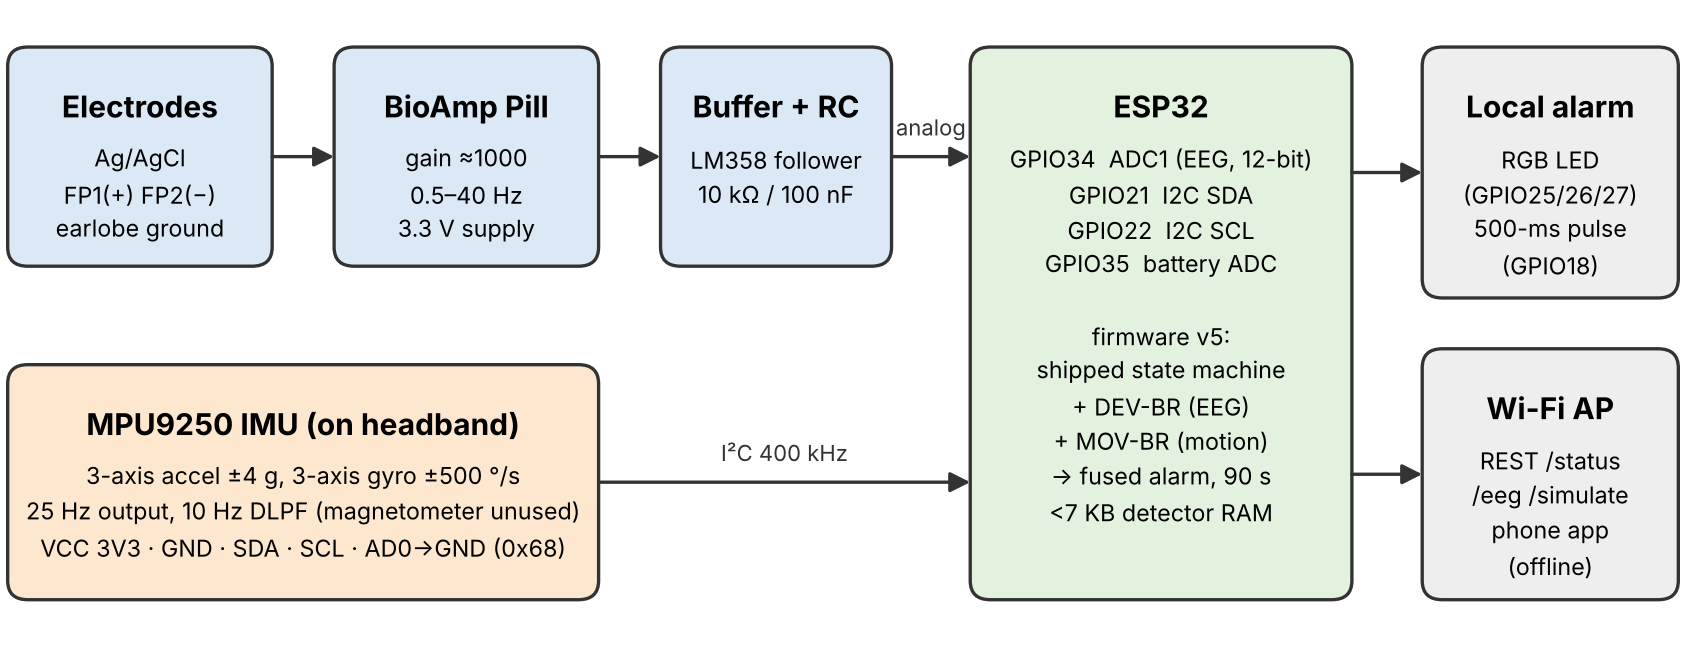
\includegraphics[width=0.8\textwidth]{figures/system_v5.png}
\caption{Prototype (firmware v5): forehead EEG via BioAmp Pill and LM358 to the ESP32 ADC; MPU9250 on the headband over I$^2$C at 25~Hz. Gain and pass-band are nominal, not measured.}
\label{fig:hw}
\end{figure*}
One forehead channel (FP1--FP2) is amplified (gain $\approx$1000, 0.5--40~Hz, 3.3~V supply; vendor documents 5~V), buffered by an LM358 (output ceiling $\approx$1.8~V at 3.3~V~\cite{lm358}) and sampled by the ESP32 at $\approx$200~Hz; an MPU9250~\cite{mpu9250} ($\pm$4~g, $\pm$500~$^\circ$/s, 10-Hz low-pass, 25~Hz) is read over I$^2$C (Fig.~\ref{fig:hw}). Table~\ref{tab:status} lists what is built, simulated and measured. Alarms drive an RGB LED, a GPIO pulse and a Wi-Fi REST API for a phone app. The MPU9250 and front-end have not been bench-characterized. The shipped (v4) firmware thresholds the deviation $d[n]{=}|x[n]-\lfloor b[n]\rfloor|$ from a 0.5-s baseline at $\mu{+}4\sigma$ of a 1-s-memory running estimate; a Python analyzer votes on line-length, delta/alpha ratio and 30--45-Hz energy.

\begin{table}[t]
\centering
\caption{Implementation status and source of each specification.}
\label{tab:status}
\footnotesize
\setlength{\tabcolsep}{2pt}
\begin{tabular}{>{\raggedright\arraybackslash}p{0.17\columnwidth}>{\raggedright\arraybackslash}p{0.43\columnwidth}>{\raggedright\arraybackslash}p{0.34\columnwidth}}
\toprule
Item & Specification & Status / source \\
\midrule
EEG front-end & Ag/AgCl FP1$+$/FP2$-$; BioAmp Pill (gain $\approx$1000, 0.5--40~Hz, 3.3~V); LM358 follower; RC 159~Hz & built; nominal values; vendor documents 5-V use~\cite{bioamp} \\
Motion sensor & MPU9250, $\pm$4~g, $\pm$500~$^\circ$/s, 10-Hz DLPF, 25~Hz, I$^2$C GPIO21/22~\cite{mpu9250} & built; not bench-characterized \\
ADC, sampling & 12-bit, default attenuation, \texttt{delay(5)} loop & firmware v5 reports measured rate \\
Outputs & RGB LED, 500-ms GPIO pulse, Wi-Fi AP REST API, phone app & firmware; app not evaluated \\
Detectors & v4: state machine + 3-feature analyzer; v5: DEV-BR, MOV-BR, co-activation & v4 replay-evaluated; v5 compiled (792~KB flash), bit-exact offline \\
Bench / human data & noise, battery, timing, wear & not measured \\
\bottomrule
\end{tabular}
\end{table}

\section{Method}\label{sec:method}
\textbf{Data.} CHB-MIT~\cite{shoeb2009thesis,goldberger2000physionet} gives the exact device montage (FP1--FP2 reconstructed from the bipolar chain; \NRec{} recordings, \NSz{} seizures, \NHours{}~h, \NSubj{} subjects) but no motion. SeizeIT2~\cite{bhagubai2025seizeit2} gives \SHours{}~h from \SNSubj{} patients with focal epilepsy: behind-the-ear EEG and a 25-Hz accelerometer on the back of the neck (\SNFBTC{} focal-to-bilateral tonic--clonic (FBTC), \SNMotor{} focal motor, \SNNonMotor{} focal non-motor and \SNOther{} other seizures; \SMovMissing{} of \SNRuns{} recordings lack motion).
\textbf{Replay.} EEG passes a causal model of the nominal front-end (0.5--40~Hz, 200~Hz, gain 1000, 12~bits); the analyzer runs unmodified on a simulated serial port and clock, and the firmware loop is ported line by line.
\textbf{Scoring.} SzCORE~\cite{dan2025szcore}: alarms within 90~s merge; detection window [onset$-$30~s, offset$+$60~s]. Parameters are chosen by leave-one-subject-out (LOSO) as the most sensitive setting meeting an FA/h target on the other subjects. CIs: subject bootstrap; tests: Wilcoxon (subjects), exact McNemar (seizures); chance: circularly shifted alarms.

\textbf{Detectors.} With $\delta(t)$ the per-second mean of $d$ and $\alpha(t)$ the per-second mean of $\lVert\mathbf a-\mathrm{EMA}_{1\,\mathrm s}(\mathbf a)\rVert$, each signal is compared with its own median over $[t{-}329,t{-}30]$: $\rho_s(t)=\log\big(s(t)/\mathrm{median}\big)$, so gain and sensor units cancel. DEV-BR (EEG) and MOV-BR (motion, optionally gated by 2--7-Hz rhythm) fire when $\rho\ge\log r$ for $D$ s. The general mode fires on EEG \emph{or} motion; the convulsive mode when $\rho_\delta\ge\log r_E$ \emph{and} $\rho_\alpha\ge\log r_M$ for $D$ s. Firmware v5 maps them to the existing BROWNOUT and BLACKOUT states with the modal LOSO parameters (convulsive: $r_E{=}4$, $r_M{=}8$, $D{=}30$~s, chosen in \SCvAParamsN{}/125 folds). It needs under 7~KB of RAM, compiles for the ESP32 (792~KB flash), and its C++ detector reproduced every evaluation alarm \SVerNote{}; it has not been timed on the device.

\begin{table*}[t]
\centering
\caption{SeizeIT2, held-out patients (LOSO) except the shipped firmware. Class columns: share of seizures of that class detected; ``Sleep'': seizures arising from sleep.}
\label{tab:s2}
\small
\setlength{\tabcolsep}{4pt}
\begin{tabular}{lcccccccc}
\toprule
Detector & Detected & Sensitivity [95\% CI] & FA/h & FBTC & Focal motor & Focal non-motor & Sleep & Chance \\
\midrule
\SMainTableBody
\bottomrule
\end{tabular}
\end{table*}

\begin{table*}[t]
\centering
\caption{CHB-MIT, FP1--FP2 (\NSubj{} subjects, \NSz{} seizures, \NHours{}~h; nominal front-end). Brackets: subject-bootstrap 95\% CI. ``Macro'': mean of per-subject sensitivities. ``Chance'': sensitivity of randomly circularly shifted alarms. BR rows: held-out subjects (LOSO).}
\label{tab:chb}
\begin{tabular}{lcccccc}
\toprule
Detector & Detected & Sensitivity [95\% CI] & Macro & FA/h & Latency (s) & Chance \\
\midrule
\MainTableBody
\bottomrule
\end{tabular}
\end{table*}

\begin{figure}[t]
\centering
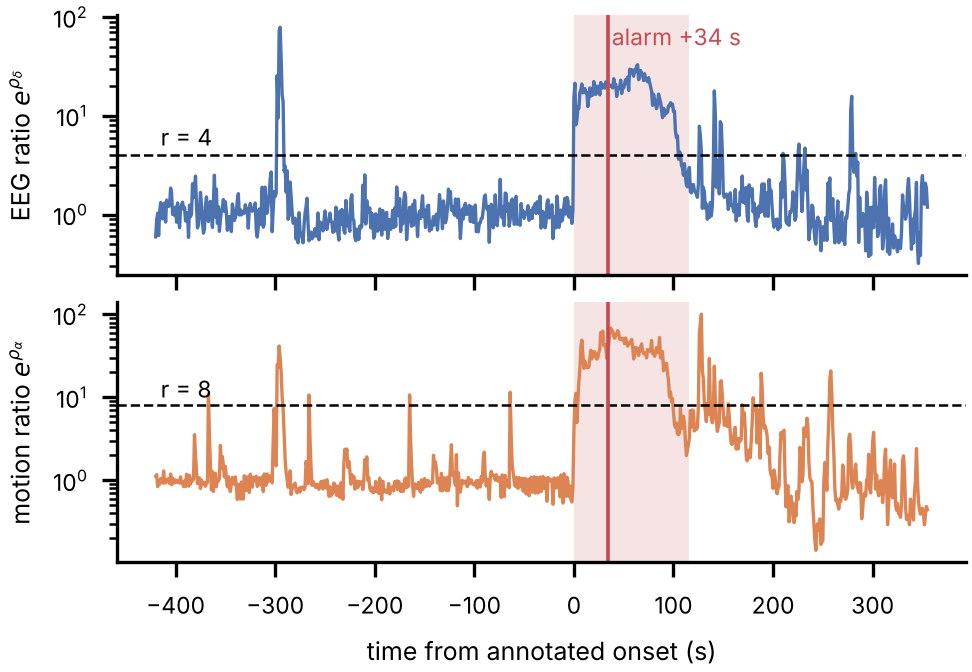
\includegraphics[width=0.95\columnwidth]{figures/convulsive_example.png}
\caption{Convulsive-mode alarm on an FBTC seizure (shaded) in SeizeIT2 patient 115, arising from sleep. Brief EEG artifacts and isolated movements cross one threshold but not both; the seizure raises both ratios and the alarm fires after the 30-s persistence. Shown: the detected sleep FBTC seizure with the shortest latency and no false alarm within 30~min (illustrative, not typical).}
\label{fig:example}
\end{figure}

\section{Results}\label{sec:res}
\textbf{CHB-MIT (device montage).} The analyzer's alarm (Table~\ref{tab:chb}) detected \PyBSens{} at \PyBFAh{}~FA/h; the firmware's \FwBSens{} at \FwBFAh{}~FA/h was largely explained by its alarm rate (chance \FwBNull{}). DEV-BR detected \DevASens{} (CI \DevACI{}) at \DevAFAh{}~FA/h, better than the analyzer in \TestDevPyBetter{} of \TestDevPyN{} subjects and worse in none (\TestDevPyP{}); unnormalized thresholds reached \AblAbsSens{}, and learned classifiers did no better. With parameters frozen it held \HwDevSensMin{}--\HwDevSensMax{} across gains of 500--2000, LM358 clipping, a 3.1-V ADC range and a 6-ms loop, while the firmware ranged \HwFwFAMin{}--\HwFwFAMax{}~FA/h (simulation).

\begin{figure*}[t]
\centering
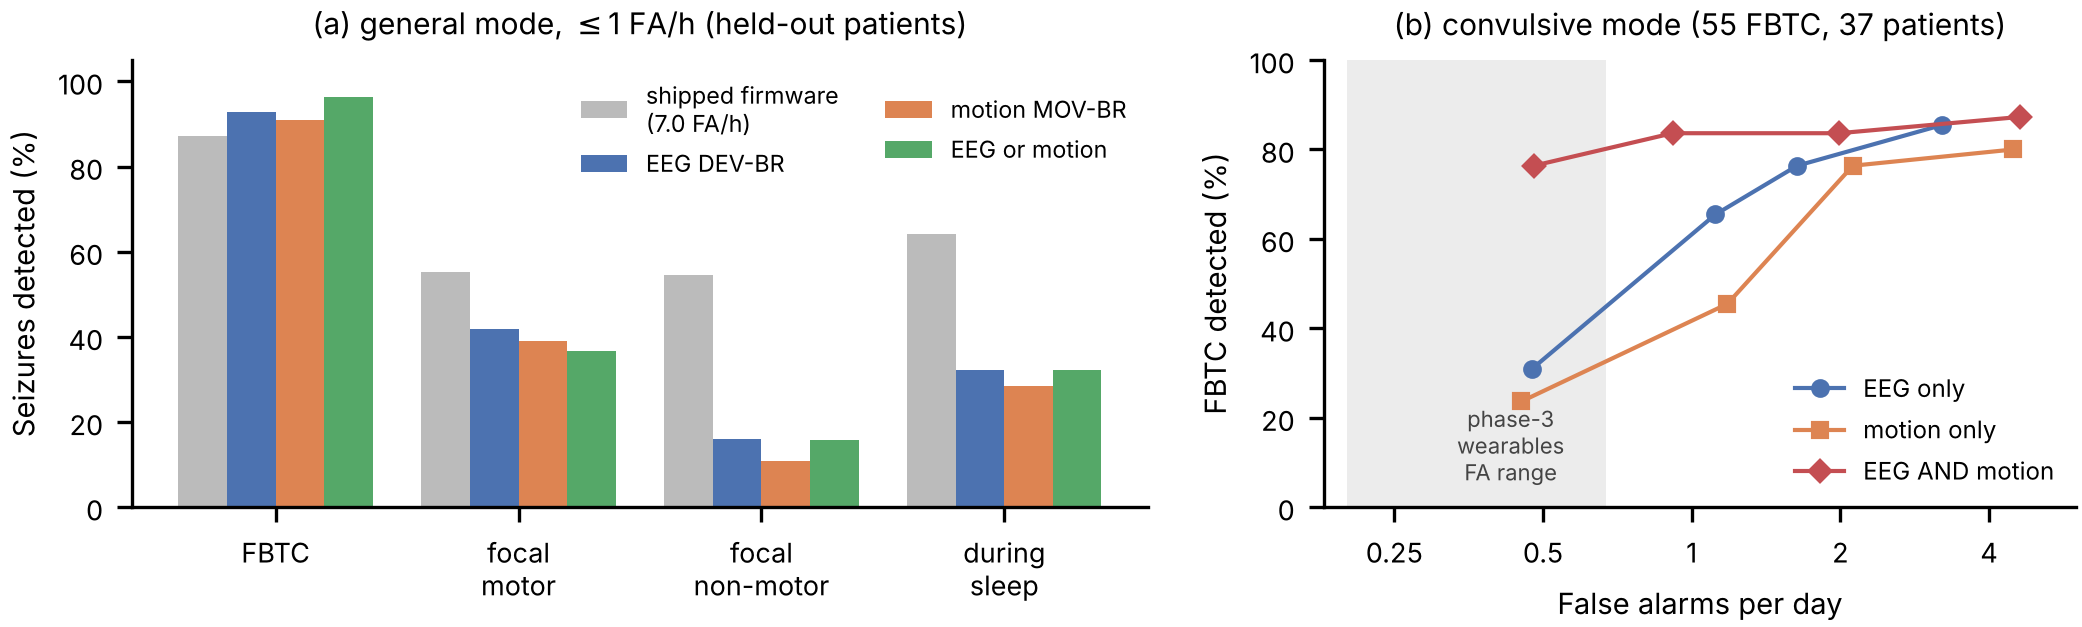
\includegraphics[width=0.86\textwidth]{figures/seizeit2_results.png}
\caption{SeizeIT2, held-out patients. (a) Seizures detected by class at $\le$1~FA/h (shipped firmware at its own 7.0~FA/h). (b) Convulsive mode: FBTC sensitivity versus false alarms per day for LOSO targets of 0.02--0.2~FA/h; shaded, the phase-3 wearable range~\cite{beniczky2021guideline}.}
\label{fig:s2}
\end{figure*}

\textbf{SeizeIT2.} The shipped firmware detected \SFwSens{} at \SFwFAh{}~FA/h (chance \SFwNull{}); at that alarm rate EEG-or-motion detected \SFusFwSens{} (\STFUSEDFwVFWBetter{} patients better, \STFUSEDFwVFWWorse{} worse, \STFUSEDFwVFWP{}). At $\le$1~FA/h, DEV-BR detected \SEegASens{} and the general mode \SFusASens{}, with large differences by class (Table~\ref{tab:s2}, Fig.~\ref{fig:s2}a): \SFusAFBTC{} of FBTC but \SFusANonMot{} of focal non-motor seizures. In convulsive mode, co-activation detected \SCvADet{}/\SCvAN{} FBTC seizures from \SCvASubj{} patients (\SCvASens{}, CI \SCvACI{}) at \SCvAFAday{} false alarms per day, \SCvASleepDet{} of \SCvASleepN{} from sleep (Fig.~\ref{fig:example}), versus \SCvEegSens{} (EEG only; McNemar \SMcEegP{}) and \SCvMovSens{} (motion only; \SMcMovP{}) at the same rate; median latency \SCvALat{}~s from the focal onset.

\section{Discussion and Conclusion}
Replaying the shipped code showed that the prototype's original alarms mostly fire at random, and one rule---compare each signal with the wearer's own delayed median---fixes the EEG detector and transfers to the MPU9250 without calibration. Adding head motion changed the result for the most dangerous seizures: neither modality alone reached a usable alarm rate, but their co-activation detected about three in four convulsive seizures inside the false-alarm range of phase-3 wearables, in under 7~KB of RAM. Performance remains below clinical devices (90--96\%~\cite{beniczky2021guideline}) and a learned model on the same data (95.5\% at 1.1/day~\cite{zhang2024multimodal}), and non-convulsive seizures are rarely caught. Limitations: results come from software replay; SeizeIT2's behind-the-ear EEG and neck-worn 25-Hz sensor differ from our forehead headband; FBTC results rest on \SCvAN{} seizures; parameters are modal LOSO choices; no bench, timing or human data are reported. Next steps are bench characterization, overnight headband recordings and an ethics-approved study. Hardware, firmware, replay code and detectors are open source~\cite{vera_repo}.

\section*{Acknowledgment}
The authors used an AI assistant (Claude, Anthropic) to help develop the code and draft the manuscript, and take full responsibility for the content.

\bibliographystyle{IEEEtran}
\bibliography{refs}

\end{document}
